\documentclass[tikz]{standalone}
\usepackage{pgfplots}
\pgfplotsset{compat=1.15}
\usepackage{mathrsfs}
\usetikzlibrary{arrows,calc}
\usepackage{tkz-euclide}
\pagestyle{empty}

\definecolor{AngleClr}{rgb}{0,0.39215686274509803,0}
\definecolor{ShapeClr}{rgb}{0.6,0.2,0}

\begin{document}

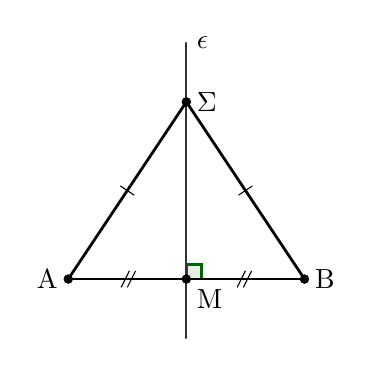
\begin{tikzpicture}[scale=.75]
\tkzSetUpLine[line width=1pt,color=black]
\tkzSetUpPoint[fill=black]

\tkzDefPoints{0/0/A,4/0/B,2/3/C,2/4/E,2/-1/D,2/0/M}

\tkzMarkRightAngle[line width=1pt, size=.25,color=AngleClr,fill=AngleClr,fill opacity=0.1](C,M,B)

\tkzDrawSegment[line width=0.8pt,color=black!80!white](E,D)
\tkzDrawSegments[line width=1.0pt,color=black](A,B A,C B,C)

\tkzDrawPoints[size=3](A,B,C,M)

\tkzLabelPoint[left](A){$\rm A$}
\tkzLabelPoint[right](B){$\rm B$}
\tkzLabelPoint[right](C){$\rm\Sigma$}
\tkzLabelPoint[below right](M){$\rm M$}

\tkzLabelSegments[pos=0.0,right](E,D){$\epsilon$}

\tkzMarkSegments[mark=s||,size=3](A,M B,M)
\tkzMarkSegments[mark=|,size=3](A,C B,C)

\end{tikzpicture}

\end{document}
